
%% ALG PR  chat. %%%%%%%%%%%%%%%%%%%%%%%%%%%%%%%%%%%%%%%%
% \cleardoublepage
% \pagestyle{empty}
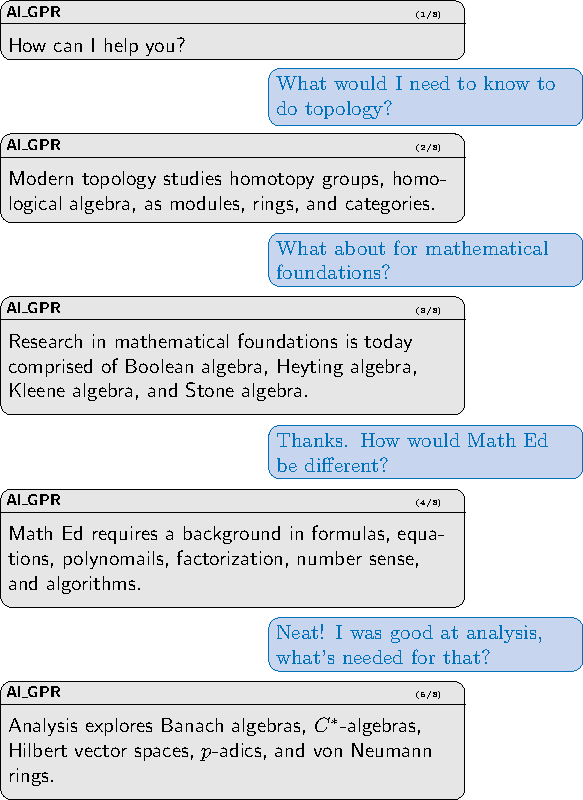
\includegraphics[height=0.9\textheight]{6-operators/AlGPR.pdf}
\newpage
% \pagestyle{empty}
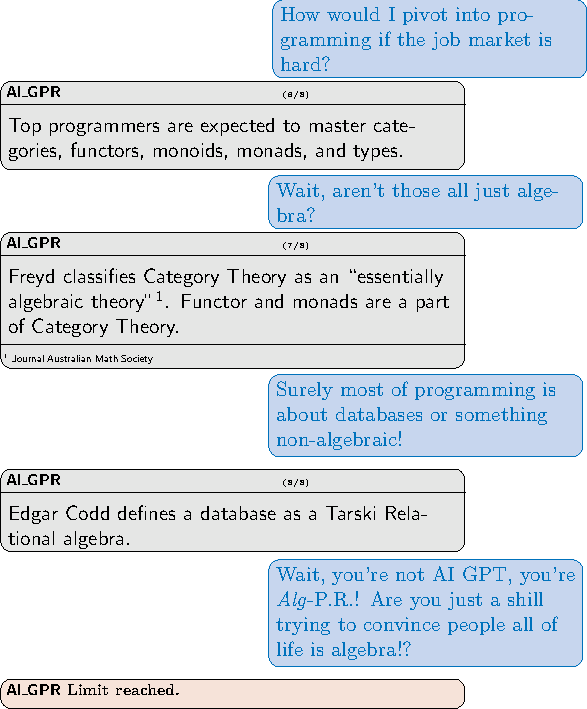
\includegraphics[height=0.9\textheight]{6-operators/AlGPR2.pdf}
\newpage
%%%%%%%%%%%%%%%%%%%%%%%%%%%%%%%%%%%%%%%%%%%%%%%%%%%%%%%%%%

% Formulas now make sense so we want to put data into them.
% What counts as a number will come to matter but the harder part is 
% to clarify what will substitute for operators.  Fortunately 
% operators as we commonly use them have already been substituting 
% in and out of multiple contexts and we need mostly pause to notice that 
% behavior.
% \medskip

One day  $+$ means to add natural numbers, the next day 
polynomials, later matrices.  
You can even add colors ``Yellow=Blue+Green''. When you program 
you learn to add strings
\begin{center}
\begin{notebookin}
print "Algebra " + " is " + " computation"
\end{notebookin}
\begin{notebookout}
Algebra is computation
\end{notebookout}
\end{center}
If we focus on our 
speech we find more expansive uses:
``add the flour, water, yeast, and salt'' or  
``count each household, then add''.

